%!TEX root = ../template.tex
\chapter{Contributions \& Planning}\label{cha:planning}

% I now propose the typestate DSL.
% This chapter goes through the “\emph{why}”, “\emph{how}” and to some extent the “\emph{when}” (i.e. the planning timeline).
% While the concept of an embedded is not novel in itself or to Rust,
% as far as I am aware, this approach to typestates is somewhat new to Rust.

\section{Objectives}

As previously discussed, the present work proposes the design of a new DSL embedded in Rust.
The core goal of the DSL is to provide typestates without getting in the way of the developer.
This means providing a syntax that stays close to Rust, only introducing new constructs when required.
Errors should be helpful and point to the original DSL code (see \autoref{lst:dsl-typestate-error}), avoiding scenarios like the “\emph{infamous}” C++ template errors.
Features should be well documented allowing anyone to get up and running quickly,
along this idea, the language itself should be a simple dependency and avoid any complicated build process.

Finally, as discussed in \autoref{sec:objectives}, the language should provide static guarantees ---
such as state usefulness and automata minimality.
That is, respectively, if a state is reachable from the start state and if it is possible to reach the end state from it;
and if the automata is minimal.
Along with usefulness checks, the presence of start and final states are also checked,
otherwise such check would not work.

\begin{align}
    Start \rightarrow A~   & ;~A \rightarrow End   \\
    Start \rightarrow End~ & ;~Start \rightarrow B \\
    Start \rightarrow End~ & ;~B \rightarrow End
\end{align}

As an example, consider the previous equations as simple state machines.
From the three, the last two would not compile as it is impossible to reach $End$ from $B$, and it is impossible to reach $B$ from $Start$, respectively.

\section{Architecture}\label{sec:arch}

The DSL should provide a specification language,
allowing the developer to describe a structure, along with possible states and functions ---
which can be pure, impure (i.e. mutating some aspect of the structure without transitioning states)
or transitions (i.e. making the transition between states).
The specification is then transformed into the necessary Rust structures and traits.
In the end, the developer should only be required to write the \keyword{impl}s for each state.

\subsection{Why function-like macros?}

In short, function-like macros allow true DSLs in Rust. However, the answer is not that simple.

\paragraph{Derive macros} seem to be a great candidate for our purpose.
We can add them to an enumeration (just like \autocite{Fitzgerald2019}) and derive the necessary states from there.
The main limitation of this approach is the lack of transparency —
the derived methods are fixed by the macro and the developer does not have control over them.

\paragraph{Attribute macros} would be an ideal candidate if we were able to tie multiple of them together.
In other words, if it was possible to relate several macro calls with each other, they could work.
This idea would be close to what Fugue \autocite{DeLine2004} does.
However, each attribute macro's scope is limited to the item it is attached to,
furthermore there is no way to store state during macro expansion in Rust.

\paragraph{Function-like macros} are the only candidate left, their capabilities enable an expressive DSL.
In comparison to the \emph{derive} approach, function-like macros provide more control and transparency to the developer.
Allowing the developer to easily control states, transitions and others.

\subsection{How does it work?}

As stated, this approach provides a DSL.
Such DSL is responsible for allowing the developer to write an expressive typestate specification.
The DSL processing is done as follows (illustrated in \autoref{fig:dsl-processing}):
\begin{compactenum}
    \item The DSL is first parsed during macro expansion.
    \item The extracted structure is converted into a state-machine.
    \item The state-machine is verified against our checks (see \autoref{sec:arch:fsm-verification}).
    \item Extract all required \keyword{trait}s and \keyword{struct}s from the specification.
    \item Expand the macro into valid Rust code.
\end{compactenum}
After this process, all that is left to do is the implementation of the \keyword{trait}s.

\begin{figure}
    \centering
    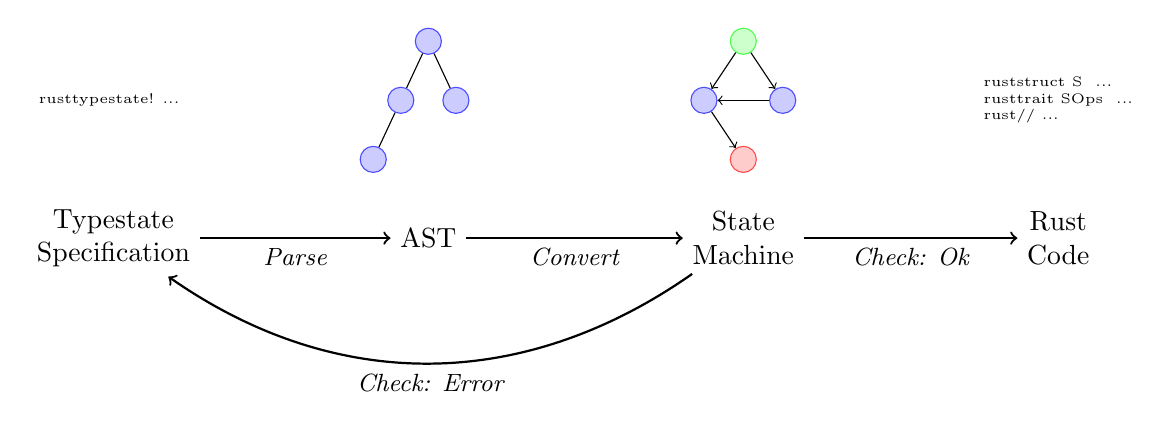
\begin{tikzpicture}
        \tikzstyle{code} = [fill=white, font=\tiny, align=left]
        \tikzstyle{phase} = [below, font=\small\itshape]

        \def\xSpec{0}
        \def\xAST{4}
        \def\xFSM{8}
        \def\xCode{12}
        \def\yLabel{-1.75}

        \node[code] (code) at (\xSpec,0) {\mintinline{rust}{typestate!{ ... }}};

        \begin{scope}[shift={(\xAST, 0.75)}]
            \tikzstyle{n}=[circle, draw=blue!70, fill=blue!20]
            \node[n] (root) at (0, 0) {};
            \node[n] (l1) at (-0.35, -0.75) {};
            \node[n] (l2) at (0.35, -0.75) {};
            \node[n] (l11) at (-0.7, -1.5) {};
            \draw[-] (root) -- (l1);
            \draw[-] (root) -- (l2);
            \draw[-] (l1) -- (l11);
        \end{scope}

        \begin{scope}[shift={(\xFSM, 0.75)}]
            \tikzstyle{n}=[circle, draw=blue!70, fill=blue!20]
            \tikzstyle{f}=[circle, draw=red!70, fill=red!20]
            \tikzstyle{s}=[circle, draw=green!70, fill=green!20]
            \node[s] (root) at (0, 0) {};
            \node[n] (l1) at (-0.5, -0.75) {};
            \node[n] (l2) at (0.5, -0.75) {};
            \node[f] (l11) at (0, -1.5) {};
            \draw[->] (root) -- (l1);
            \draw[->] (root) -- (l2);
            \draw[->] (l1) -- (l11);
            \draw[->] (l2) -- (l1);
        \end{scope}

        \node[code] (rust-code) at (\xCode,0) {\mintinline{rust}{struct S { ... }}\\\mintinline{rust}{trait SOps { ... }}\\\mintinline{rust}{// ...}};

        % \draw[->, thick] (code) -> (2.5, 0);
        % \draw[->, thick] (4.5, 0) -> (5, 0);
        % \draw[->, thick] (7, 0) -> (rust-code);

        \node[align=center] (label-1) at (\xSpec, \yLabel) {Typestate\\Specification};
        \node[align=center] (label-2) at (\xAST, \yLabel) {AST};
        \node[align=center] (label-3) at (\xFSM, \yLabel) {State\\Machine};
        \node[align=center] (label-4) at (\xCode, \yLabel) {Rust\\Code};

        \draw[->, thick] (label-1) -- node[phase] {Parse} (label-2);
        \draw[->, thick] (label-2) -- node[phase] {Convert} (label-3);
        \draw[->, thick] (label-3) -- node[phase] {Check: Ok} (label-4);
        \draw[->, thick] (label-3) edge[in=-35, out=-145] node[phase] {Check: Error} (label-1);

    \end{tikzpicture}
    \caption{
        From DSL specification to Rust code.
        First the DSL is parsed, then converted to a state machine and its properties checked
        (in the some property is not respected, an error is issued).
        Once the properties are validated, the Rust code is generated.
    }
    \label{fig:dsl-processing}
\end{figure}

\subsection{Syntax}\label{sec:arch:syntax}

% One of the DSL's syntax goals is to stay as close to Rust as possible.
The macro is invoked through a \keyword{typestate!} call, inside it, lives the DSL.
I go through some important aspects, such as state and function declaration syntax.
\autoref{lst:dsl-typestate-spec} is an example of the full syntax.

\paragraph{The top-level declaration} names the typestated output structure (line 1 of \autoref{lst:dsl-typestate-spec}).
It starts with a name, the structure identifier, and a pair of curly brackets containing the specification.
While this syntax would allow for multiple declarations to be written,
the macro call can be become unnecessarily complex if several declarations are allowed inside.

\paragraph{A state declaration} uses the \keyword{struct} keyword (lines 2-7 of \autoref{lst:dsl-typestate-spec}).
The choice of \keyword{struct} over \keyword{state} is based on the following reasons:
\begin{compactitem}
    \item Keeping the syntax close to Rust by avoiding a new keyword.
    \item Each state boils down to a structure, hence it is a natural mapping made explicit.
    \item Since the code inside the DSL already implies typestates, each structure can easily be thought of as a state.
    This follows the previous point idea.
\end{compactitem}

\paragraph{A function declaration} shares the syntax with their Rust counterparts (lines 12-18 of \autoref{lst:dsl-typestate-spec}).
They can be one of three possible categories:
\begin{compactitem}
    \item \keyword{pure} functions, which do not mutate state (e.g. line 12 of \autoref{lst:dsl-typestate-spec}).
    Their signature takes an immutable reference to \keyword{self} as an argument,
    disabling mutation.
    \item \keyword{impure} functions, which can mutate state but not transition between states (e.g. line 13 of \autoref{lst:dsl-typestate-spec}).
    Their signature takes a mutable reference to \keyword{self} as an argument.
    This allows for mutation of the current state, but not transition.
    \item \keyword{transition} functions, which transition between states (lines 14-18 of \autoref{lst:dsl-typestate-spec}).
    Their signature takes ownership of \keyword{self},
    forcing the consumption of the current state disabling possible aliasing.
\end{compactitem}
These keywords can be explicit, but they can also be inferred from the code.
% Along with the keyword distinction, the \keyword{self} parameter is now typed.
% This represents a change to original Rust's syntax, although a required one.
% The alternative would be to specify the state parameter inside brackets,
% which in comparison with the typed-\keyword{self} approach is less natural.
The reader may have noticed two details in \autoref{lst:dsl-typestate-spec} ---
the \texttt{Flying} state is not used,
the \texttt{fly\_to} function returns the same state as \keyword{self}.
This is the case since the function will make the transition between \texttt{Hovering}, \texttt{Flying} and back internally.
Thus requiring \keyword{self} to be consumed.



\paragraph{Initial and final states} are special cases as they are defined with both structures and functions.
The syntax to declare initial and final states is presented in lines 16-17 of \autoref{lst:dsl-typestate-spec}.
As the reader can observe, the syntax uses functions to declare with states are initial and final.
Both can also be inferred using the following rules:
\begin{compactitem}
    \item \textbf{Initial states} are declared with functions that do not take \keyword{self} as a parameter and return a state.
    The \keyword{self} keyword is omitted since the state is yet to be built.
    \item \textbf{Final states} are declared as “\emph{consumers}”, that is, they take \keyword{self} as a parameter and do not return a value.
    This syntax makes clear that the state becomes unavailable for further processing.
\end{compactitem}

\paragraph{Non-deterministic transitions} are useful to cover cases where the output is dependent on some external factors.
Consider a process that can fail, the developer is required to model both the success and failure cases.
To do so, the developer can declare an \keyword{enum}, containing possible outcomes.
Such enumeration has one key difference from regular Rust enumerations, the fields must contain existing states only,
that is, structures declared inside the same macro call (lines 8-11 and 15 of \autoref{lst:dsl-typestate-spec}).
Enforcing these transitions can either be done by leveraging Rust's enumerations and leaving the matching up to the user,
or through determinization of the automata.

\begin{listing}
    \centering
    \begin{minted}{rust}
typestate! { Drone {
    struct Grounded { location: Coordinates }
    struct Hovering { location: Coordinates }
    struct Flying {
        location:    Coordinates,
        destination: Coordinates,
    }
    enum Landed {
        Success(Grounded),  // houston, touchdown!!
        Error,              // crashed
    }
    fn get_location(&self: Grounded) -> &Coordinates;
    fn correct_coordinates(&mut self: Grounded);
    fn take_off(self: Grounded) -> Hovering;
    fn fly_to(self: Hovering, dst: Coordinates) -> Hovering;
    fn land(self: Hovering) -> Landed;
    fn new() -> Grounded;   // defines the start state
    fn end(self: Grounded); // defines the final state
} }
    \end{minted}
    \caption{
        Example specification of the \texttt{Drone} typestate using the proposed DSL.
    }
    \label{lst:dsl-typestate-spec}
\end{listing}

\begin{listing}
    \centering
    \begin{minted}{text}
typestate! { Drone {
    struct State;
           ^^^^^ : error `State` is not a useful state
} }
    \end{minted}
    \caption{
        Example error issued by the DSL.
    }
    \label{lst:dsl-typestate-error}
\end{listing}

\begin{listing}
    \centering
    \begin{minted}{rust}
trait DroneState {}
struct Grounded { location: Coordinates }
impl DroneState for Grounded {}
struct Drone<State: DroneState> { state: State }
trait GroundedOps {
    fn get_location(&self) -> &Coordinates;
    fn take_off(self) -> Drone<Hovering>;
}
    \end{minted}
    \caption{
        Example generated Rust code for the \texttt{Grounded} state.
        Notice the \texttt{DroneState} trait, its purpose is to bound valid drone states.
        The trait should follow the sealed trait pattern, but it was simplified in this example.
    }
    \label{lst:dsl-typestate-generated}
\end{listing}


\begin{listing}
    \centering
    \begin{minted}{rust}
impl GroundedOps for Drone<Grounded> {
    fn take_off(self) -> Drone<Hovering> { /* ... */ }
}
    \end{minted}
    \caption{
        To make the drone usable, the developer must implement the generated traits.
        In this case, only the \texttt{Grounded} state is considered.
    }
    \label{lst:dsl-typestate-impl}
\end{listing}

\subsection{State-Machine Conversion}
The reader might have noticed that the specification syntax cleanly maps to a state machine.
As discussed in \autoref{sec:arch:syntax}, each \keyword{struct} is a state and each function is either a transition or a function which does not change state.
From the code, we can establish states as nodes and functions as edges,
effectively converting the specification into automata.

\subsection{State-Machine Verification}\label{sec:arch:fsm-verification}
After extraction the state-machine is subject to verification,
this process is done using existing algorithms \autocite{Hopcroft2013}, to check the following properties:
\begin{compactitem}
    \item \textbf{Minimality.} The state machine should be minimal in the sense that there should be no redundancy in states and transitions.
    \item \textbf{Non-empty language.} Ensuring the presence of final states.
    \item \textbf{Usefulness.} As discussed, all states should be reachable from the start state and be able to reach the end state.
\end{compactitem}
In this case, the user should get feedback over any infraction,
explaining the reasoning behind the error or warning.

\subsection{Developer Workflow}
The final user workflow should be as follows:
\begin{compactenum}
    \item The developer starts by writing the specification, as in \autoref{lst:dsl-typestate-spec}.
    \item When done, the developer compiles the code.
    In turn, the compiler will begin the process of expanding the macro.
    This process is illustrated in \autoref{fig:dsl-processing}.
    \begin{compactitem}
        \item During expansion, if the state machine fails any of the verifications described in \autoref{sec:arch:fsm-verification},
        a compiler error is issued.
        \item If no errors are reported, the process continues as normal and generates all required boilerplate, like in \autoref{lst:dsl-typestate-generated}.
        This boilerplate does not appear for the user, hence it is required the generation process is as predictable as possible.
    \end{compactitem}
    \item After generation, the user is now required to implement all functions, as in \autoref{lst:dsl-typestate-impl}.
\end{compactenum}


\section{Previously Developed Work}

Currently, I have developed a really simple proof-of-concept macro for Rust typestates.
The macro is based on declarative macros and has several limitations,
its syntax is also distant from the current proposal.
The macro takes a simple typestate specification and expands into several traits and structures.
This project can be found on GitHub \autocite{Duarte2020a}.

\subsection{Improvement Points}

As it stands, the project has several possible improvement points to be addressed during the development phase.
Such points are as follows:
\begin{compactitem}
    \item The macro's syntax does not support functions. This implies that it does not support transitions.
    \item The fact that the macro is written using declarative macros makes the underlying code complex and barely readable.
    This is due to the fact that declarative macros are not suited for bigger scale macros.
    \item The macro does not verify state-machine properties, such as the previously enumerated, reachability and termination.
    \item The supported syntax adds new language constructs, such as the \keyword{limited} and \keyword{strict} keywords.
    \item The macro only supports “\emph{phantom}” states, that is, states do not hold any data
    (the name comes from Rust's \keyword{PhantomData}, which is used to implement these kind of states).
\end{compactitem}



